\documentclass[cal1spr16Lectures.tex]{subfiles}

\begin{document}

%\section[]{}%[Week 10]{Week 10: 28 Mar - 1 Apr}

% % % 
\subsubsection{\bf Wednesday 30 March}
% % %

\begin{frame}[allowframebreaks]{Wed 30 Mar}
\begin{itemize}%\footnotesize
\item Exam 3: next Friday.  Covers \S 3.10-4.6
\item Algebra Seminar: today at 3p in SCEN 322.

``The talk will be given by our own Ashley Wheeler on the 

Title:  Local cohomology of Stanley-Reisner rings." (from the department email). 
\end{itemize}
\end{frame}

% % %
\subsection[4.4 Optimization Problems]{\S 4.4 Optimization Problems}
% % %

% % %
\begin{frame}{\S 4.4 Optimization Problems}
\small
In many scenarios, it is important to find a maximum or minimum value under given constraints.  Given our use of derivatives from the previous sections, optimization problems follow directly from what we have studied.
\end{frame}

% % %
\begin{frame}
\frametitle{}
\small
\begin{que} Given all nonnegative real numbers $x$ and $y$ between 0 and 50 such that their sum is 50 (i.e., $x+y=50$), which pair has the maximum product? \end{que}

\vspace{2pc}
This is a basic optimization problem.  In this problem, we are given a \alert{\bf constraint} ($x+y=50$) and asked to maximize an \alert{\bf objective function} ($A=xy$).
\end{frame}

% % %
\begin{frame}
\frametitle{}
\small
The first step is to express the objective function $A=xy$ in terms of a \alert{single variable} by using the constraint:
\[y=50-x \implies A(x)=x(50-x).\]

\vspace{2pc}
To maximize $A$, we find the critical points:
\[A^{\prime}(x)=50-2x\ \text{which has a critical point at}\ x=25.\]
\end{frame}

% % %
\begin{frame}
\frametitle{}
Since $A(x)$ has domain $[0,50]$, to maximize $A$ we evaluate $A$ \alert{at the endpoints of the domain and at the critical point}:
\[A(0)=A(50)=0\ \text{and}\ A(25)=625.\]

\vspace{2pc}
So 625 is the maximum value of $A$ and $A$ is maximized when $x=25$ (which means $y=25$).
\end{frame}

% % %
\subsubsection{Essential Feature of Optimization Problems}
% % %

% % %
\begin{frame}{\small Essential Feature of Optimization Problems}
\small
All optimization problems take the following form:
\begin{center}
\alert{\it What is the maximum (or minimum) value of an objective function subject to the given constraint(s)?}
\end{center}

\vspace{2pc}
Most optimization problems have the same basic structure as the previous problem:  An objective function (possibly with several variables and/or constraints) with methods of calculus used to find the maximum/minimum values.
\end{frame}

% % %
\begin{frame}
\frametitle{}
\small
\begin{exe} Suppose you wish to build a rectangular pen with two interior parallel partitions using 500 feet of fencing.  What dimensions will maximize the total area of the pen?
\begin{center}
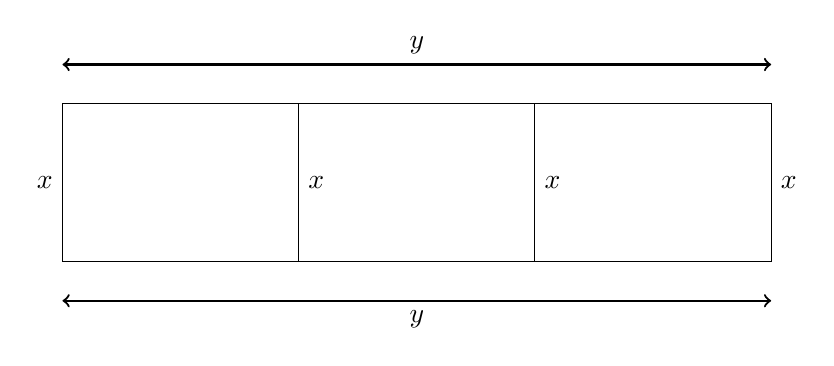
\begin{tikzpicture}
\draw (0,0) -- (3,0) 
   -- (3,2) node[midway,right] {$x$}
	 -- (0,2)
   -- (0,0) node[midway,left] {$x$};
\draw (3,0) -- (6,0)
	 -- (6,2) node[midway,right] {$x$}
	 -- (3,2)
	 -- (3,0);
\draw (6,0) -- (9,0)
	 -- (9,2) node[midway,right] {$x$}
	 -- (6,2)
	 -- (6,0);
\draw [<->] [thick] (0,-0.5) -- (9,-0.5) node[midway,below] {$y$};
\draw [<->] [thick] (0,2.5) -- (9,2.5) node[midway,above] {$y$};
\end{tikzpicture}
\end{center}
\end{exe}
\end{frame}

% % %
\begin{frame}
\small
By the picture, $2y+4x=500$ which implies $y=-2x+250$.  We are maximizing $A=xy$.  So write
\[A(x)=x(-2x+250)=-2x^2+250x.\]

Taking the derivative, $A^{\prime}(x)=-4x+250=0$, $A$ has a critical point at $x=62.5.$
\end{frame}

% % %
\begin{frame}
\footnotesize
From the picture, since we have $500$ ft of fencing available we must have $0 \le x \le 125$.  To find the max we must examine the points $x=0,62.5,125$:
\[A(\alert{0})=A(\alert{125})=0\text{ and }A(\alert{62.5})=7812.5\]

\vspace{1pc}
We see that 
\[\boxed{\text{the maximum area is}\ 7812.5\ \text{ft}^2.}\]
The pen's dimensions (answer the question!) are $\boxed{x=62.5\ \text{ft}}$ and 
\[\boxed{y=-2(62.5)+250=125\ \text{ft}.}\]
\end{frame}

% % %
\subsubsection{Guidelines for Optimization Problems}
% % %

% % %
\begin{frame}{\small Guidelines for Optimization Problems}
\footnotesize
\begin{itemize}
\item[1.] \alert{READ THE PROBLEM} carefully, identify the variables, and organize the given information with a picture.
\item[2.] Identify the objective function (i.e., the function to be optimized).  Write it in terms of the variables of the problem.
\item[3.] Identify the constraint(s).  Write them in terms of the variables of the problem.
\item[4.] Use the constraint(s) to eliminate all but one independent variable of the objective function.  
\item[5.] With the objective function expressed in terms of a single variable, find the interval of interest for that variable.
\item[6.] Use methods of calculus to find the absolute maximum or minimum value of the objective function on the interval of interest.  If necessary, \alert{check the endpoints}.
\end{itemize}
\end{frame}

% % %
\begin{frame}
\begin{que}
The sum of a pair of positive real numbers that have a product of 9 is 
\[S(x) = x + \frac{9}{x},\]
where $x$ is one of the numbers.  This sum $S(x)$ has a minimum when:
\begin{itemize}
\item[A. ] $x=9$
\item[B. ] $x=3$
\item[C. ] $x=6$
\item[D. ] none of the above
\end{itemize}
\end{que}
\end{frame}

% % %
\begin{frame}%[t]
\frametitle{}
\small
\begin{exe} An open rectangular box with square base is to be made from $48\ \text{ft}^2$ of material.  What dimensions will result in a box with the largest possible volume? \end{exe}

\vspace{1pc}
\begin{exe} Find the dimensions of the rectangle of largest area which can be inscribed in the closed region bounded by the $x$-axis, $y$-axis, and the graph of $y=8-x^3$. \end{exe}
\end{frame}

% % %
\subsubsection{Book Problems}

% % %
\begin{frame}
\begin{block}{4.4 Book Problems}
5-16, 19-20, 24, 26 
\end{block}
\end{frame}

\end{document}